% =============================
% ภาคผนวก
% =============================
% หมายเหตุ: ก่อนเริ่มภาคผนวก ระบบจะสร้างหน้าคั่นให้อัตโนมัติ
% ใช้คำสั่ง \appendiceschapter{ชื่อภาคผนวก} สำหรับแต่ละภาคผนวก
% ระบบจะกำหนดตัวอักษร ก, ข, ค ... ให้โดยอัตโนมัติ
% =============================
% ภาคผนวก ก
% =============================
\setcounter{chapter}{-1}
\appendiceschapter{ภาพหน้าจอระบบ}
\section*{ภาพหน้าจอระบบ}

ภาคผนวกนี้แสดงภาพหน้าจอการทำงานของระบบทั้งหมดที่พัฒนาขึ้น เพื่อให้เห็นภาพรวมของการออกแบบส่วนติดต่อกับผู้ใช้

\begin{figure}[H]
\centering
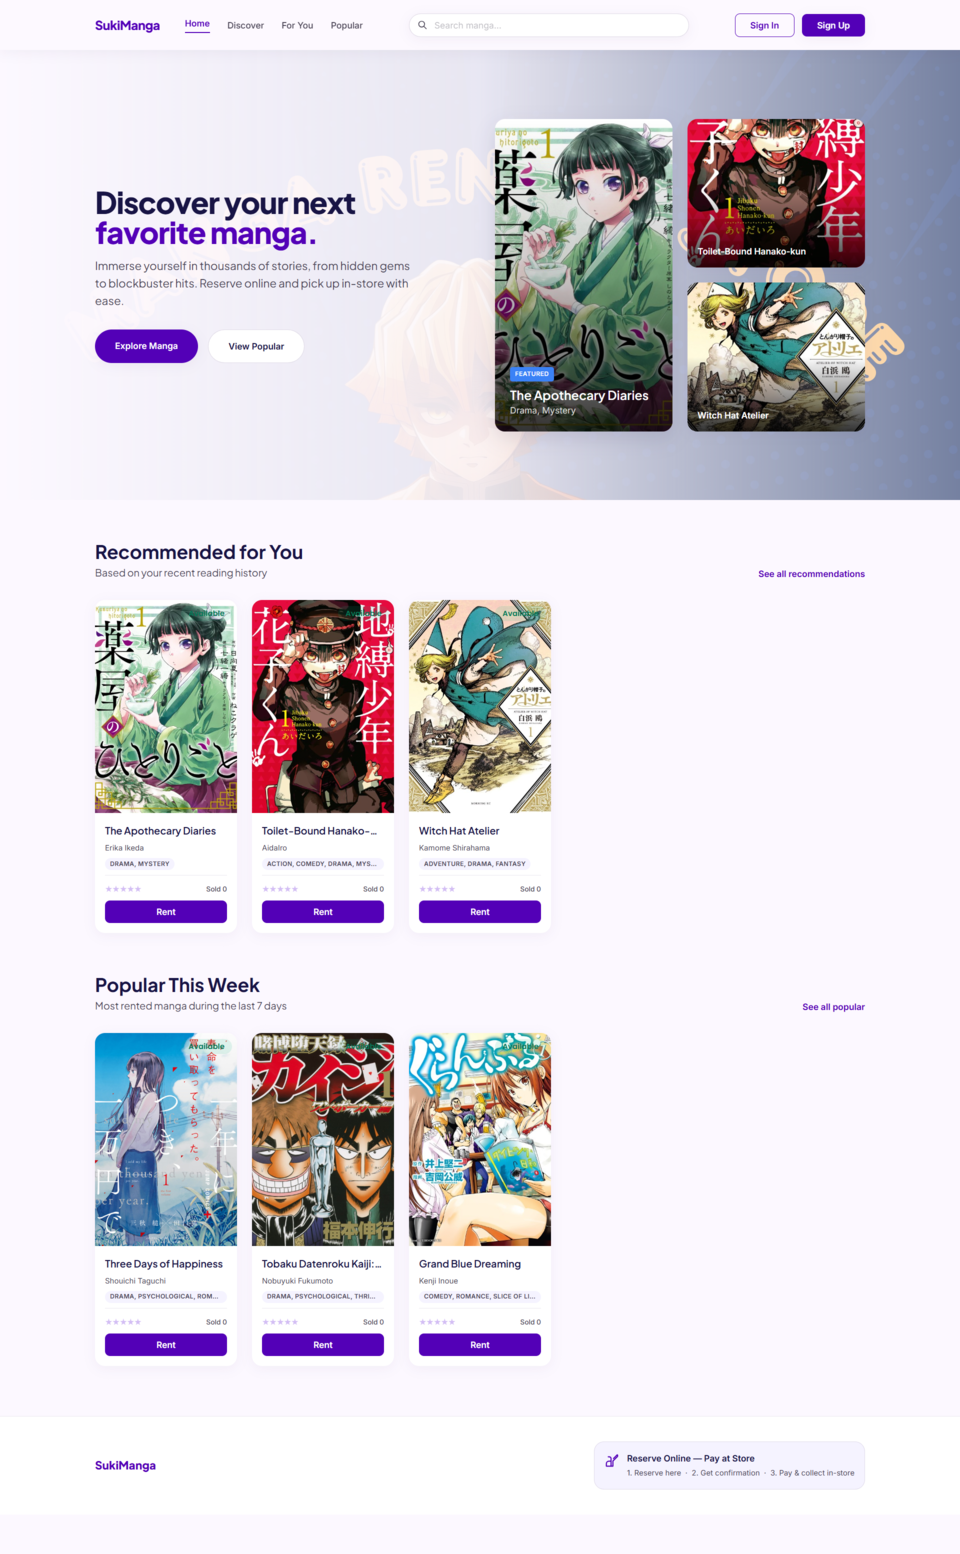
\includegraphics[width=0.8\textwidth]{images/landingPage.png}
\caption{หน้า Landing Page}
\label{fig:app_landingpage}
\end{figure}

\begin{figure}[H]
\centering
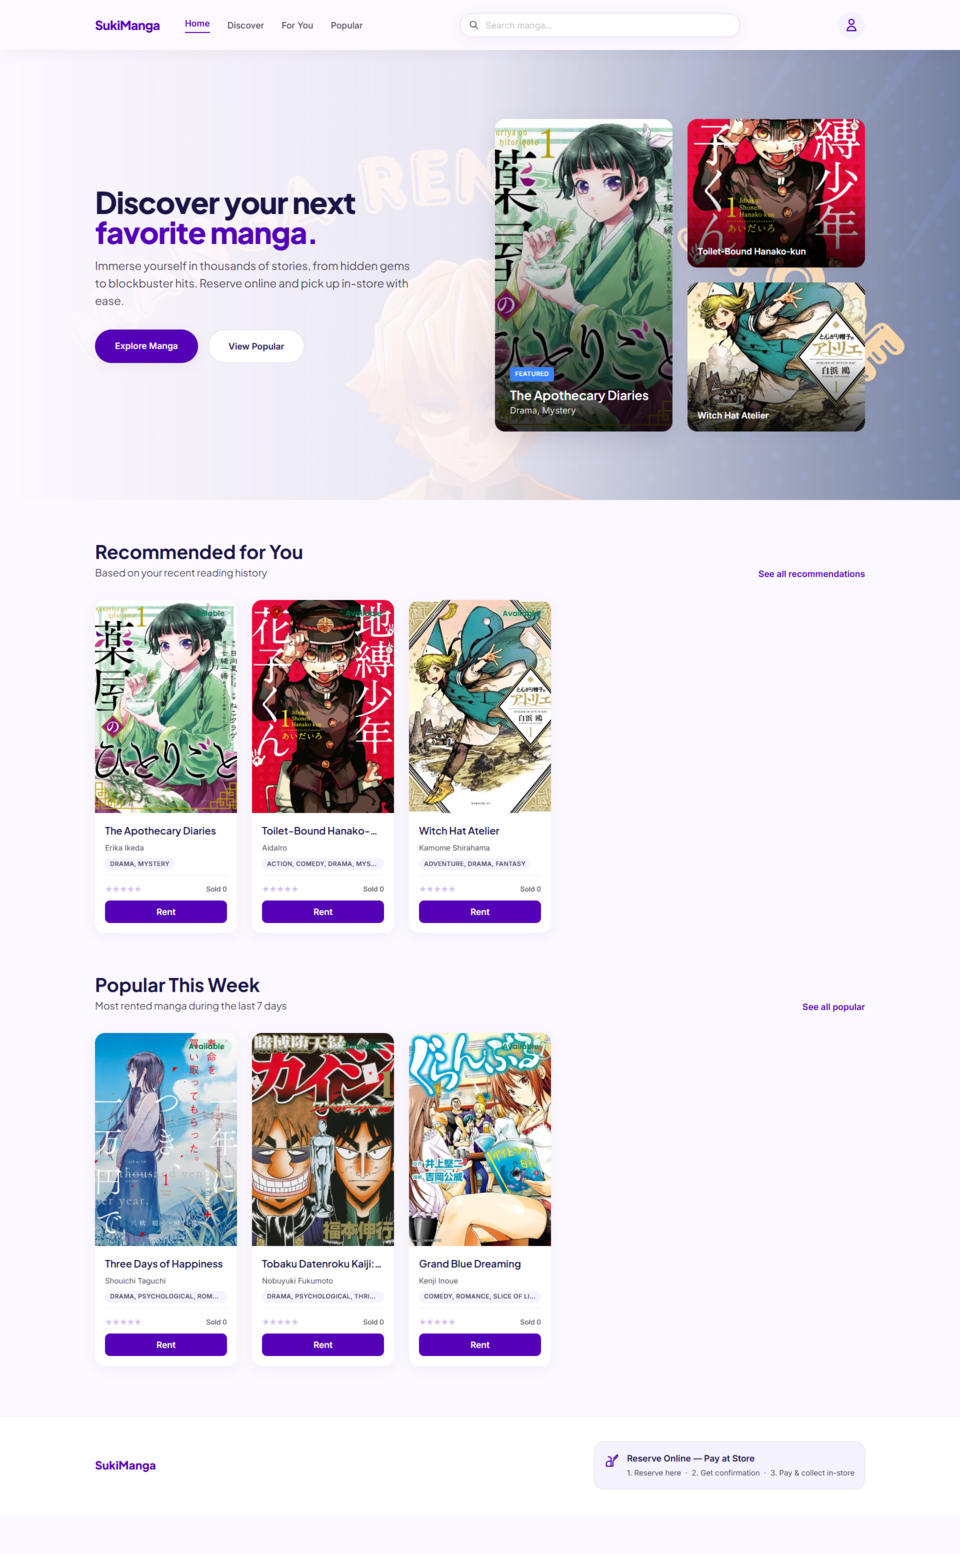
\includegraphics[width=0.8\textwidth]{images/landingPageaftersignin.png}
\caption{หน้า Landing Page หลังเข้าสู่ระบบ}
\label{fig:app_landingaftersignin}
\end{figure}

\begin{figure}[H]
\centering
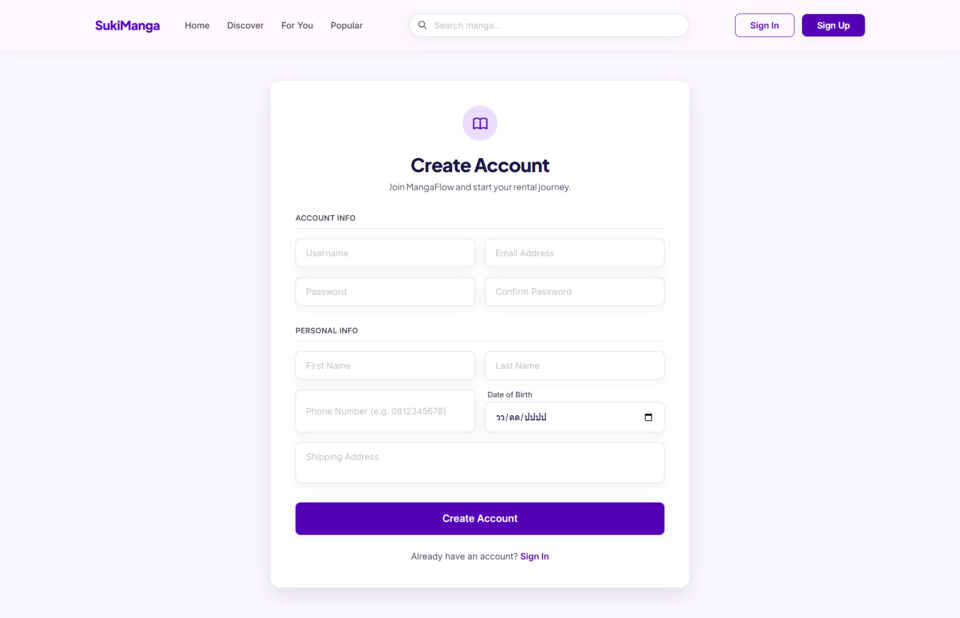
\includegraphics[width=0.8\textwidth]{images/signup.png}
\caption{หน้าสมัครสมาชิก}
\label{fig:app_signup}
\end{figure}

\begin{figure}[H]
\centering
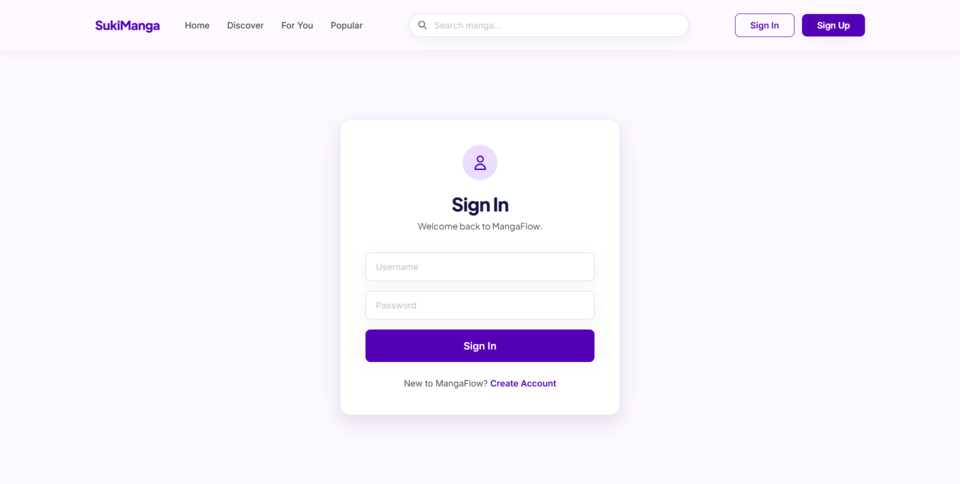
\includegraphics[width=0.8\textwidth]{images/signin.png}
\caption{หน้าเข้าสู่ระบบ}
\label{fig:app_signin}
\end{figure}

\begin{figure}[H]
\centering
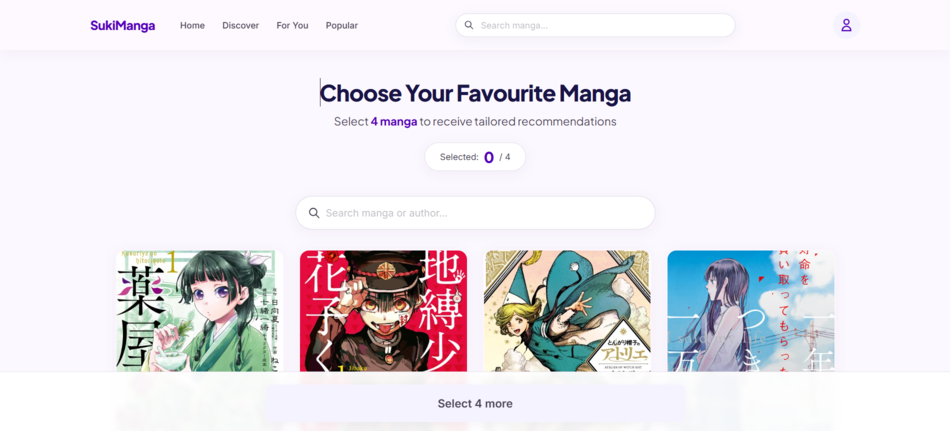
\includegraphics[width=0.8\textwidth]{images/chooseyourfav.png}
\caption{หน้าเลือกแนวการ์ตูนที่สนใจ}
\label{fig:app_chooseurfav}
\end{figure}

\begin{figure}[H]
\centering
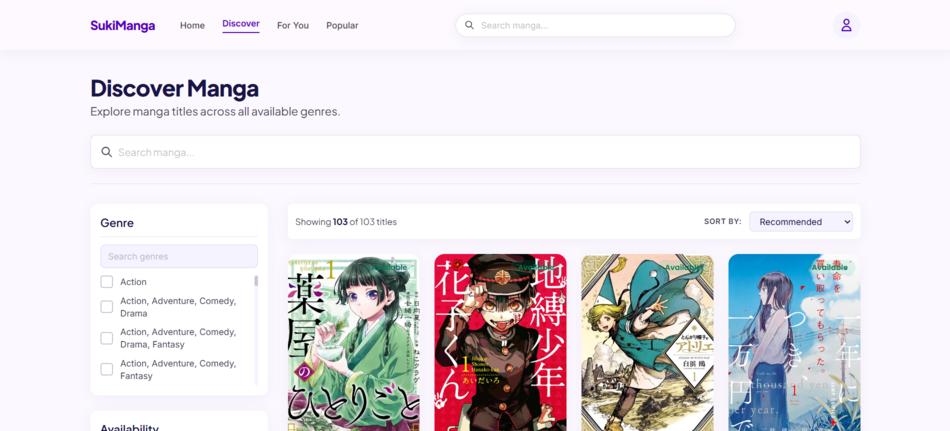
\includegraphics[width=0.8\textwidth]{images/discover.png}
\caption{หน้าค้นหาและสำรวจหนังสือ}
\label{fig:app_discover}
\end{figure}

\begin{figure}[H]
\centering
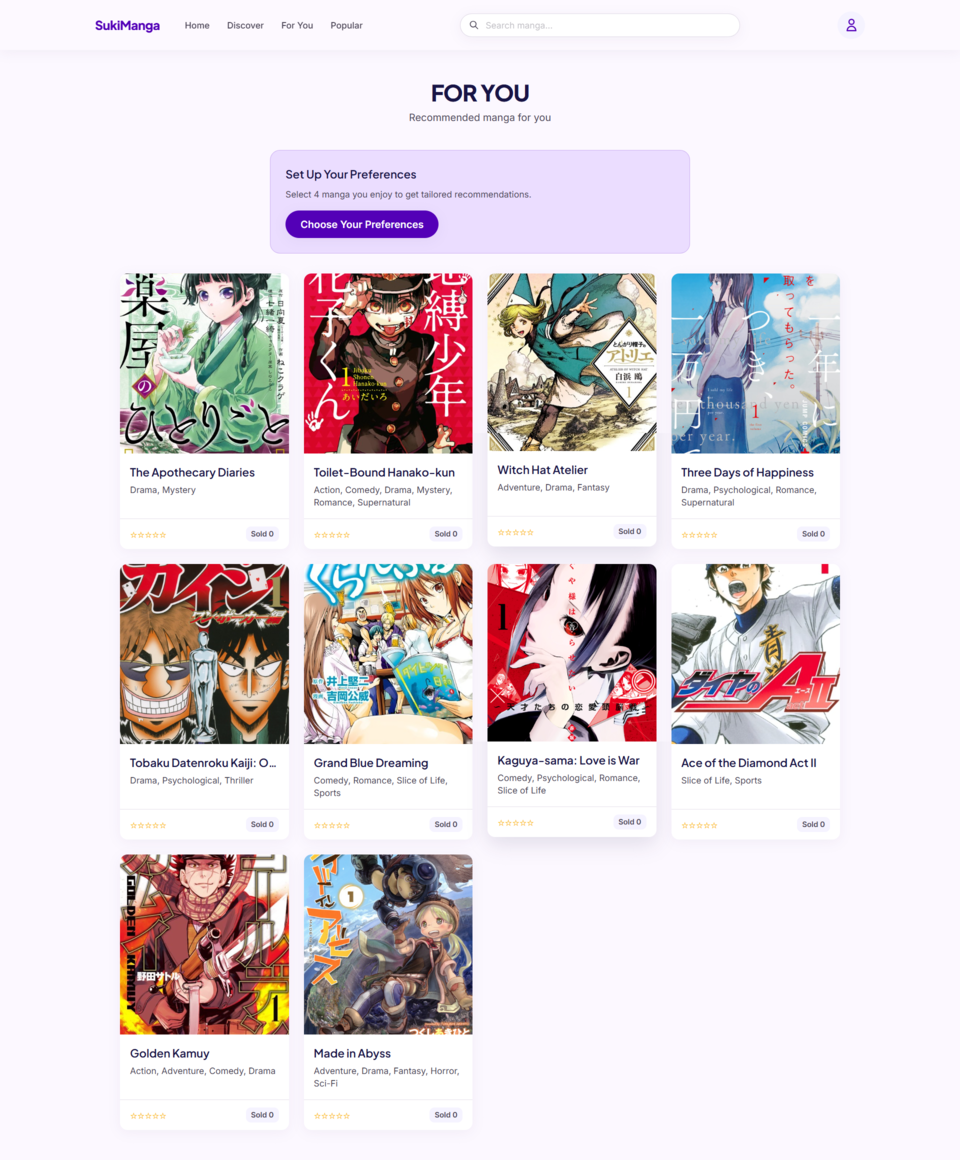
\includegraphics[width=0.8\textwidth]{images/foryou.png}
\caption{หน้าแนะนำหนังสือสำหรับคุณ}
\label{fig:app_foryou}
\end{figure}

\begin{figure}[H]
\centering
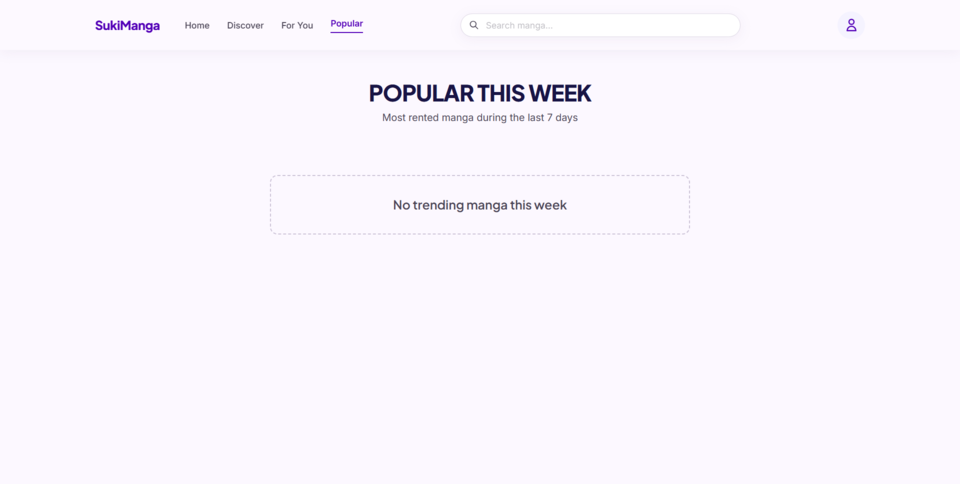
\includegraphics[width=0.8\textwidth]{images/popular.png}
\caption{หน้าหนังสือยอดนิยม}
\label{fig:app_popular}
\end{figure}

\begin{figure}[H]
\centering
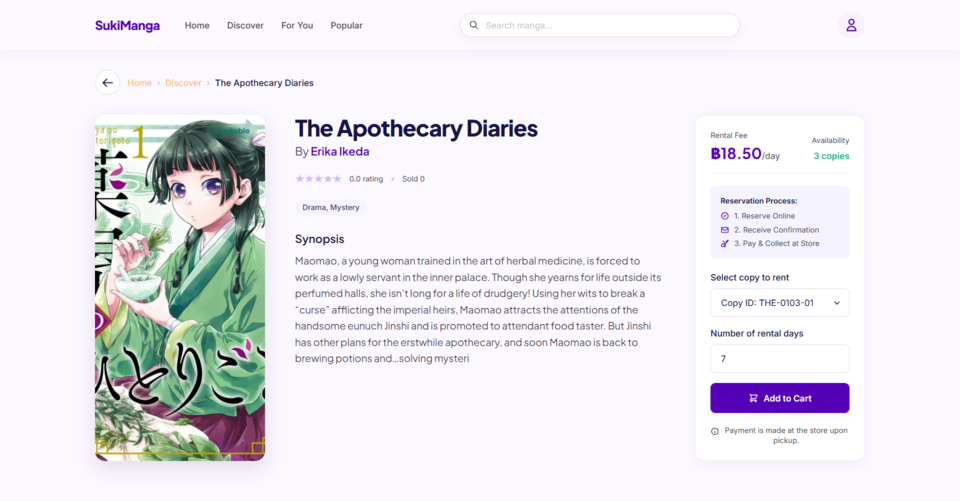
\includegraphics[width=0.8\textwidth]{images/detailManga.png}
\caption{หน้าดูรายละเอียดหนังสือ}
\label{fig:app_detailmanga}
\end{figure}

\begin{figure}[H]
\centering
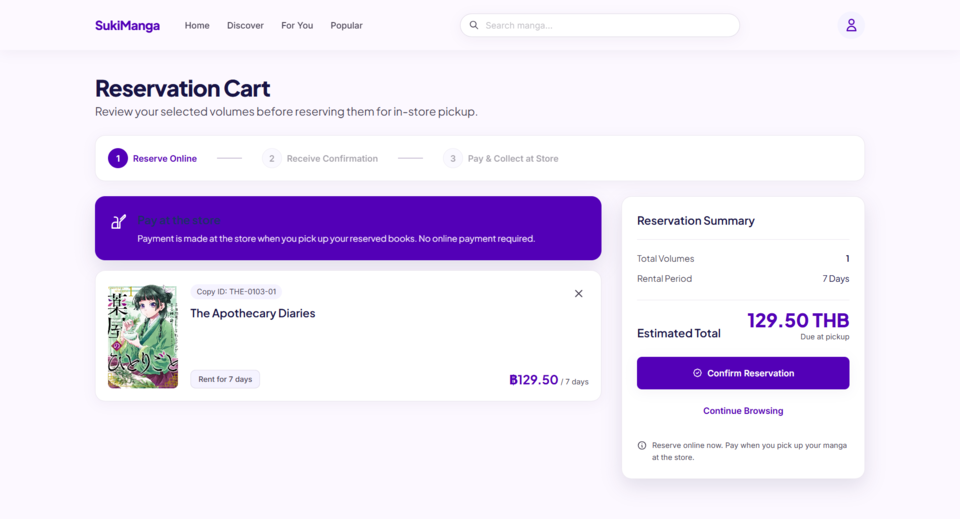
\includegraphics[width=0.8\textwidth]{images/myCart.png}
\caption{หน้าแสดงรายการที่อยู่ในตะกร้า}
\label{fig:app_mycart}
\end{figure}

\begin{figure}[H]
\centering
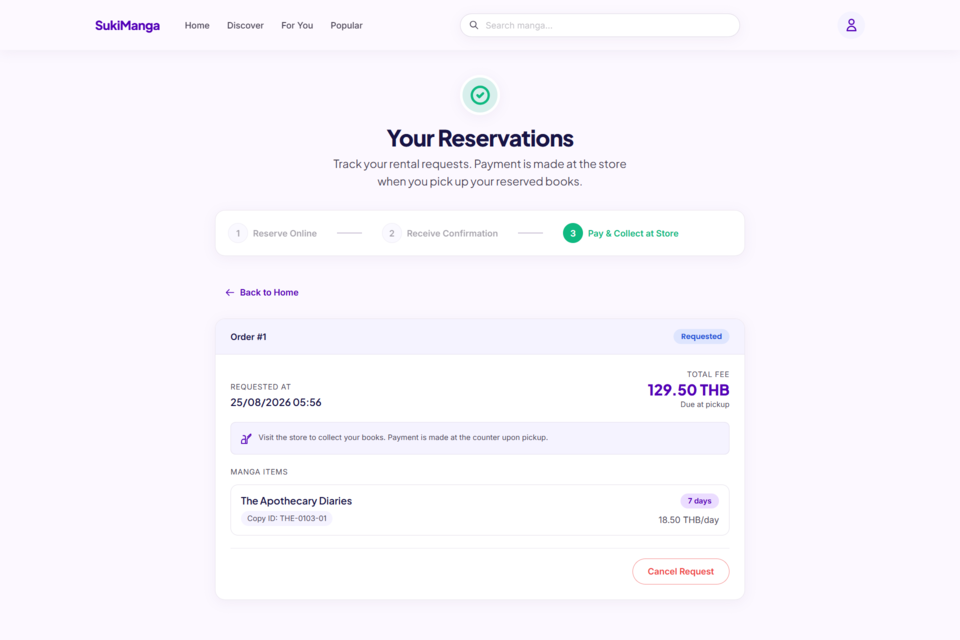
\includegraphics[width=0.8\textwidth]{images/reservationsuccess.png}
\caption{หน้าแจ้งเตือนเมื่อทำการเช่าสำเร็จ}
\label{fig:app_reservationsuccess}
\end{figure}

\begin{figure}[H]
\centering
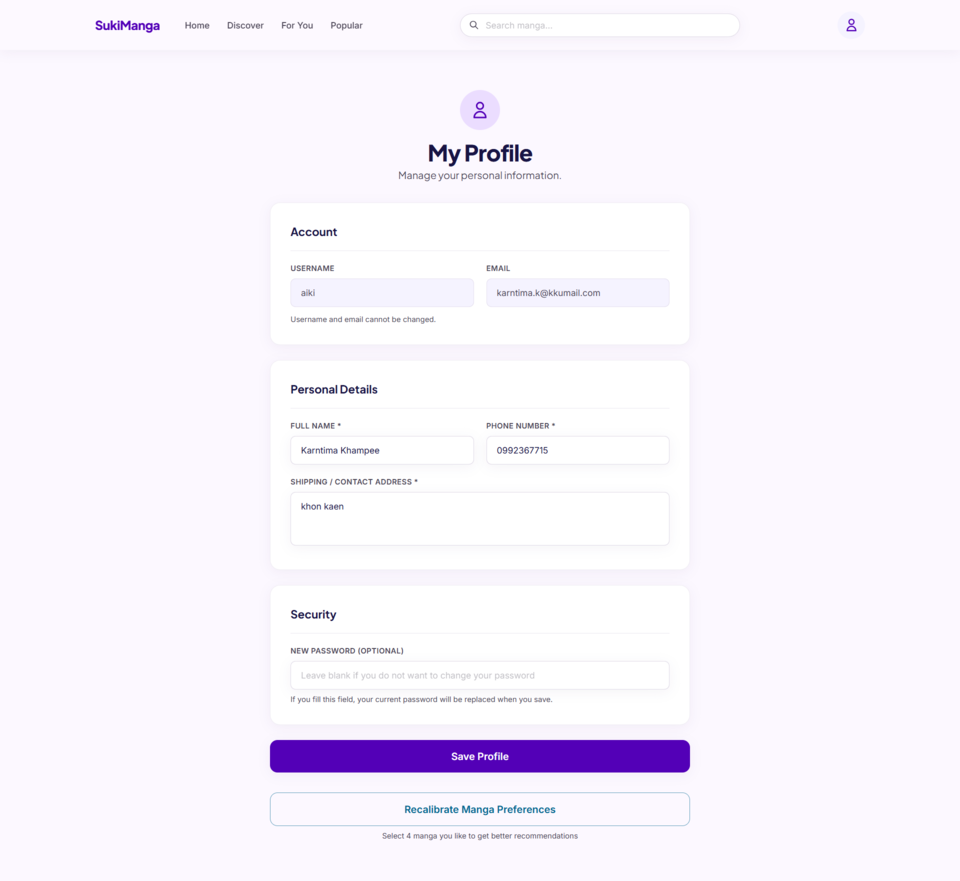
\includegraphics[width=0.8\textwidth]{images/myProfile.png}
\caption{หน้าโปรไฟล์ของผู้ใช้}
\label{fig:app_myprofile}
\end{figure}

\begin{figure}[H]
\centering
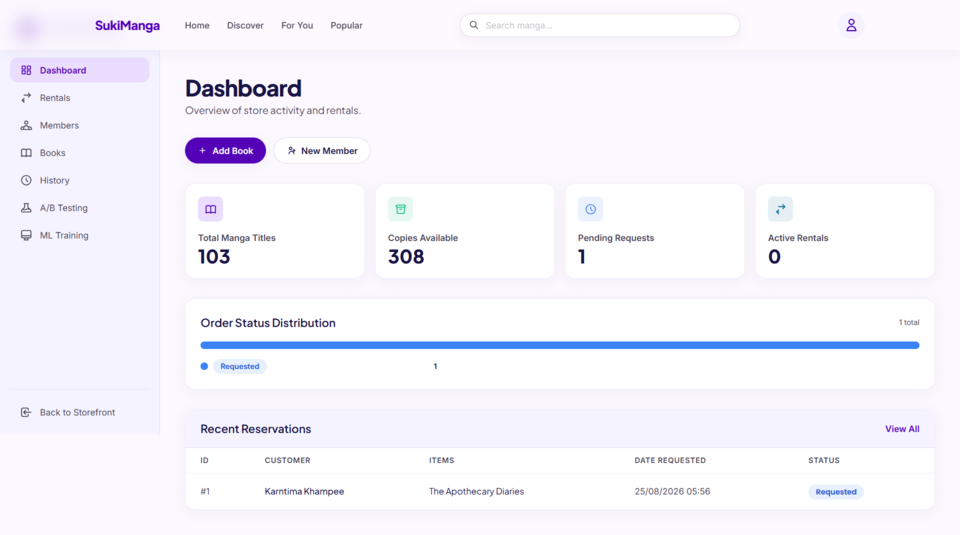
\includegraphics[width=0.8\textwidth]{images/adminDashboard.png}
\caption{หน้าแอดมิน Dashboard}
\label{fig:app_admindashboard}
\end{figure}

\begin{figure}[H]
\centering
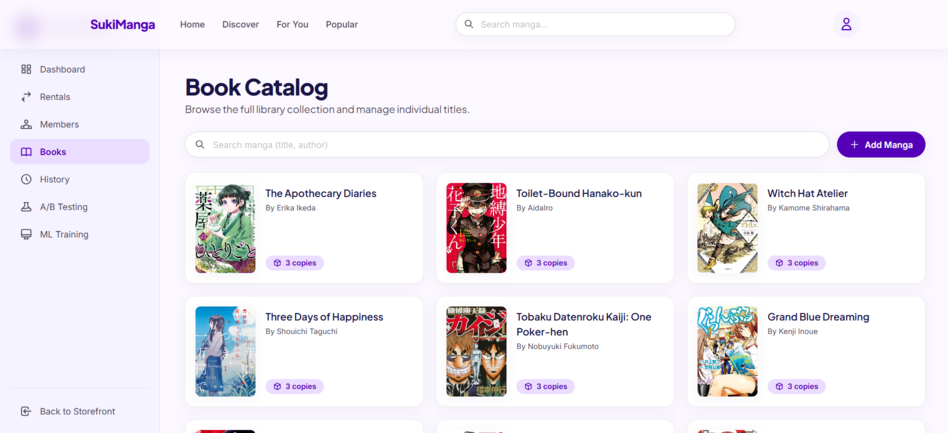
\includegraphics[width=0.8\textwidth]{images/adminManageBook.png}
\caption{หน้าจัดการรายการหนังสือ}
\label{fig:app_adminmanagebook}
\end{figure}

\begin{figure}[H]
\centering
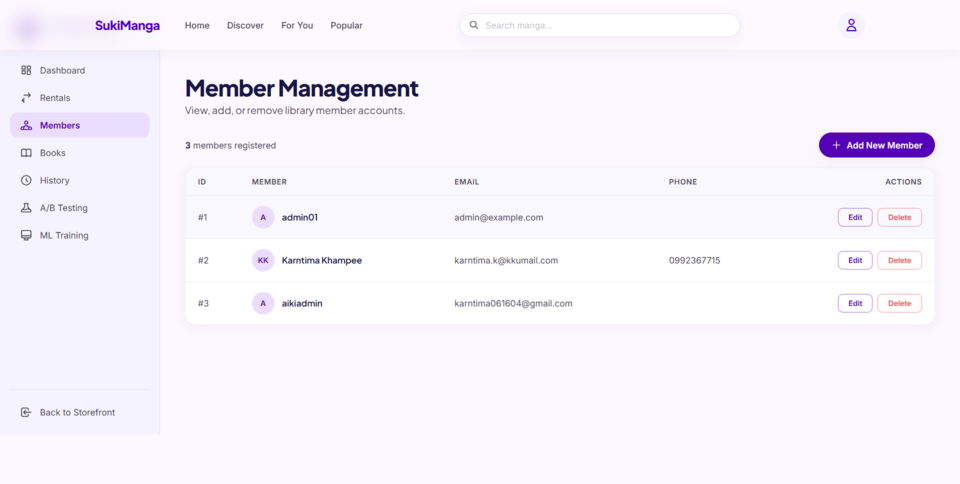
\includegraphics[width=0.8\textwidth]{images/adminManageMember.png}
\caption{หน้าจัดการสมาชิกผู้ใช้}
\label{fig:app_adminmanagemember}
\end{figure}

\begin{figure}[H]
\centering
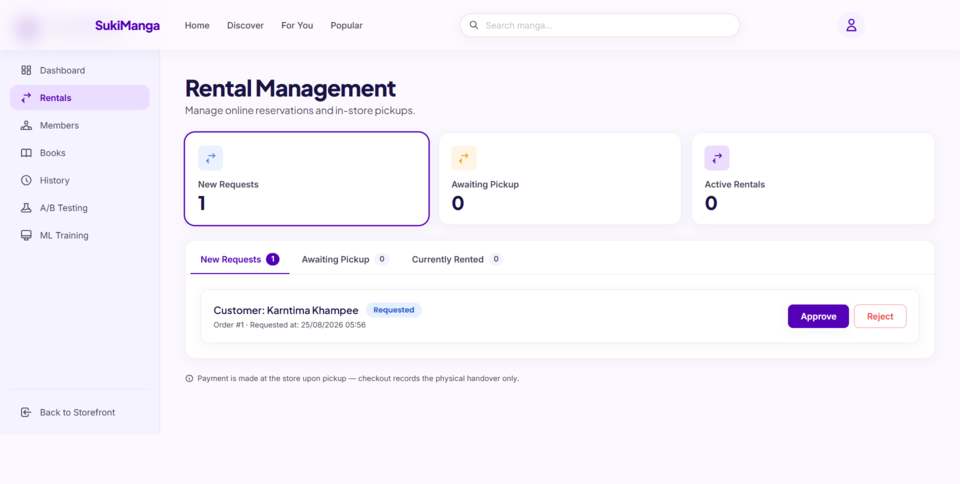
\includegraphics[width=0.8\textwidth]{images/adminManageRental.png}
\caption{หน้าจัดการรายการเช่าของแต่ละสถานะ}
\label{fig:app_adminmanagerental}
\end{figure}

\begin{figure}[H]
\centering
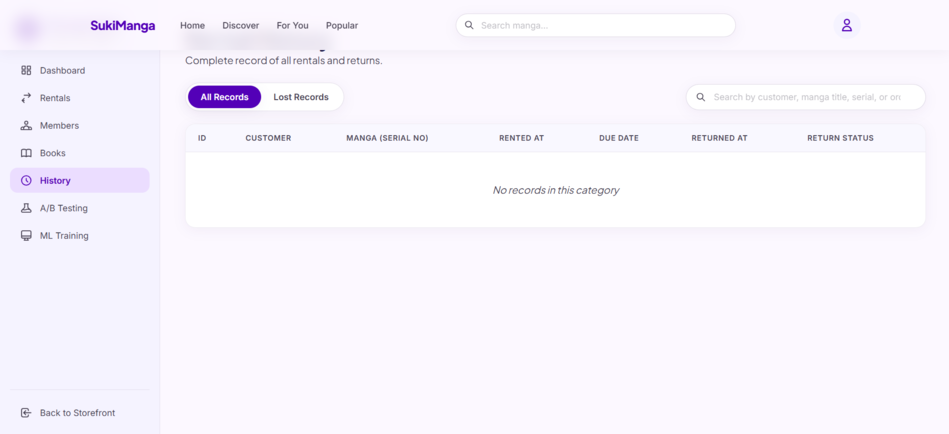
\includegraphics[width=0.8\textwidth]{images/adminViewHistory.png}
\caption{หน้าแสดงประวัติการเช่า}
\label{fig:app_adminviewhistory}
\end{figure}

\begin{figure}[H]
\centering
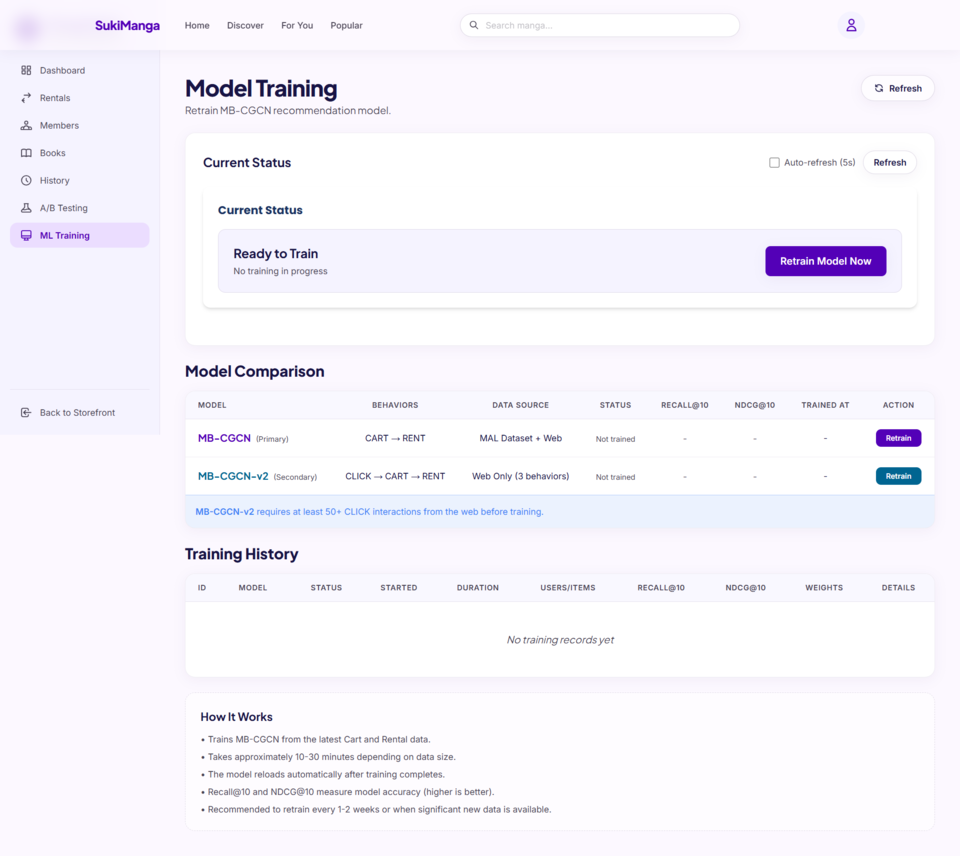
\includegraphics[width=0.8\textwidth]{images/adminMLTraining.png}
\caption{หน้าฝึกสอนโมเดลระบบแนะนำ}
\label{fig:app_adminmltraining}
\end{figure}

\begin{figure}[H]
\centering
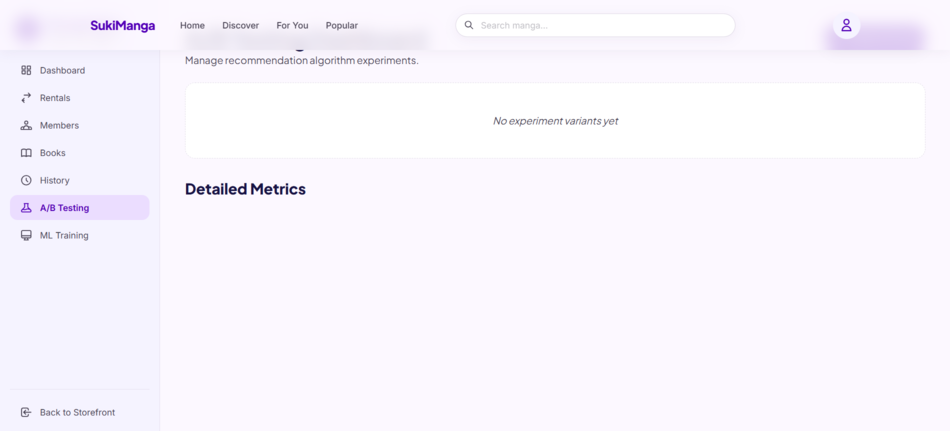
\includegraphics[width=0.8\textwidth]{images/adminABTesting.png}
\caption{หน้าการทดสอบแบบ A/B Testing}
\label{fig:app_adminabtesting}
\end{figure}

% =============================
% ภาคผนวก ข (ตัวอย่าง — uncomment ถ้าต้องการ)
% =============================
% \appendiceschapter{รายละเอียดเพิ่มเติม}
% \section*{หัวข้อ}
% เนื้อหาภาคผนวก ข